\documentclass[12pt]{article}
\usepackage[T1]{fontenc}
\usepackage[utf8]{inputenc}
\usepackage{palatino}
\usepackage{tipa}
\usepackage[dvipsnames]{xcolor}
\usepackage{arydshln}
\usepackage{tikz}
\usepackage{mathtools}
\usetikzlibrary{decorations.pathreplacing}
\usetikzlibrary{matrix}
\usepackage[round]{natbib}
\def\bibfont{\small}
\setcitestyle{aysep={}}
\usepackage{gb4e}
\renewcommand\labelitemi{--}
\newcommand{\ts}{\textsigma}
\newcommand{\tom}{\textomega}
\newcommand{\tsc}{\textsc}
\newcommand{\sig}{\sigma}
\newcommand{\tip}{\textipa}
\newcommand{\deq}{\stackrel{d}{=}}
\newcommand{\ass}{\acute{\sig}}
\newcommand{\acl}{\acute{L}}
\newcommand{\ach}{\acute{H}}
\newcommand{\tm}{\textnormal}
\newcommand{\tr}{\ass\sig}
\newcommand{\im}{\sig\ass}
\newcommand{\brass}{{\color{BrickRed}{\ass}}}
\begin{document}

\begin{center}
{\LARGE The computational nature of stress assignment} \\
\vspace{1em}
Nate Koser \\
Phonology Seminar\\
Rutgers University \\
Spring 2019
\end{center}

%combine 2.1 and 2.2 we know that all qflfp definable functions are sequential and sequential relevant to phonology, etc cite adam and jane's paper on qflfp and sequential 

%bounded QS are basically QF look in Hayes


\section{Introduction}

This paper examines stress assignment as a function from a logical, computational perspective. Assuming that a stress assignment function takes as its input a string of bare syllables and outputs a string of syllables marked with stress, what is the appropriate logical characterization of this mapping, and what does this tell us about the nature of the computation? I show that most stress assignment is describable by a \textit{least fixed point logic} (LFP) \citep{libkin04} that is restricted to be \textit{quantifier free} (QF).

All functions definable with this QFLFP logic belong to the \textit{sequential} class of functions of Formal Language Theory \citep{chandJardSeq}. The sequential class is important for phonology, as many attested phonological patterns fall within this boundary, while unattested, non-phonological patterns do not \citep{heinzlai13}. Interestingly, while all \textit{quantity insensitive} (QI) stress patterns fall within the sequential class of functions, some \textit{quantity sensitive} (QS) stress patterns provably exceed this boundary, showing that not all stress assignment is equal in terms of computational complexity. This is not an advocation of or claim specific to any particular theory of stress -- it is an empirical fact of the computation.

In examining these patterns, I take \citet{kager07} and \citet{gordon2002} as a general guide to stress typology. The definitions of the functions described abstract away from foot structure \citep{hayes95} or the metrical grid \citep{libprin77}, though I reference parsing to feet when doing so is convenient. 

\section{Logical maps}

\subsection{Model theoretic representations of stress}

In this paper stress assignment is characterized as a function from strings of bare syllables (or Ls (light) and Hs (heavy) in QS languages) to a string of syllables marked with stress. This is done in terms of logical transductions from a model-theoretic input signature to an output signature. 

To demonstrate, say we wanted to represent an input string of four syllables. We have a model with a domain $\mathcal{D}$, a set comprised of four elements; a unary relation $P_\sig$, a set of elements whose members are labeled as syllables; and two functions $p$ (predecessor) and $s$ (successor) that describe the ordering of the elements in the model. This gives us the following model and string model representation of the sequence $\sig\sig\sig\sig$:

\begin{exe}
\item 

 $\langle \mathcal{D}; P_\sig,p, s\rangle \; \mathcal{D}=\{1,2,3,4\}; \: P_\sig = \{1,2,3,4\}; \;p = x-1, s = x+1$ \\ 


 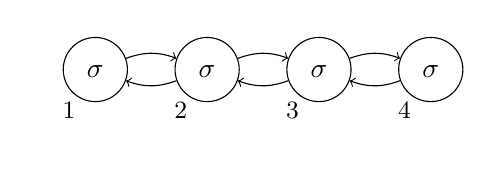
\begin{tikzpicture}[->, baseline=(m-1-1.base)]
    \matrix (m)
    [matrix of nodes, column sep=.75em, %row sep = -.3em,
     nodes={circle,text height=.75em, text depth = 2pt, text width = 1em, draw, align=center}]
    {
      \node(m-1-1)[label={[label distance=-.5em]260:{\small $1$}}]{$\sig$}; &
      \node(m-1-2)[label={[label distance=-.5em]260:{\small $2$}}]{$\sig$}; &
      \node(m-1-3)[label={[label distance=-.5em]260:{\small $3$}}]{$\sig$}; &
      \node(m-1-4)[label={[label distance=-.5em]260:{\small $4$}}]{$\sig$}; \\
    };
    \path(m-1-1) edge[bend left=20] (m-1-2);
    % \draw(m-1-1) to [bend left=45] (m-1-3);
    % \draw(m-1-1) to [bend left=45] (m-1-4);
    \path(m-1-2) edge[bend left=20]  (m-1-3);
    % \draw(m-1-2) to [bend right=45] (m-1-4);
    \path(m-1-3) edge[bend left=20]  (m-1-4);
    \path(m-1-4) edge[bend left=20]  (m-1-3);
    \path(m-1-3) edge[bend left=20]  (m-1-2);
    \path(m-1-2) edge[bend left=20]  (m-1-1);
  \end{tikzpicture}
 \label{exmodel}
\end{exe}

\noindent
Then we can use the \textit{signature} over the model -- a fixed set of relations -- to talk about any string of input syllables:

\begin{exe}
\item $S = \lbrace P_\sig, \; s, \; p \rbrace $
\end{exe}

\noindent
In addition to the model, we also have a logic that allows us to make statements about the facts of the models and string representations they describe. The logic is a formal language comprised of a set of atomic formulae that are the relations and functions in our model. The atomic formulae take variables that are interpreted with regard to a specific model. For example, if $P_\sig(x)$ is an atomic formula in some model, then it is true when $x$ is interpreted as some element $d \in P_\sig$ in that model. In the model above in (\ref{exmodel}), $P_\sig(x)$ is true for all four elements, as they are all syllables i.e. in the set of the unary relation $P_\sig$.

Given a logic and a model, we can also define logical transductions \citep{courcelle94} that describe functions from an input structure to an output structure by defining the relations of the output signature in terms of the relations and logic of the input signature. For stress assignment, this means adding a unary relation, $P'_\ass$ in the output signature and specifying when a position in the output string should be labeled with that unary relation using the logic of the signature. 

Suppose we wanted to describe an ``initial stress'' function - a function that takes an input string of syllables and returns an output structure where the first syllable is labeled as stressed. An example of this kind of stress assignment is found in Nenets \citep{decsy66}. To describe this transduction, we define each relation in the output signature $S' = \lbrace P'_\ass, \; P'_\sig, \; s', \; p' \rbrace$ in terms of the input signature $S = \lbrace P_\sig, \; s, \; p \rbrace $: 

\begin{exe}
\item $\begin{array}{l}
   P'_\ass(x) \deq  p(x) \approx x  \\
   P'_\sig(x) \deq  \neg p(x) \approx x  \\
   s'(x) \deq s(x)    \\
   p'(x) \deq p(x)
     
\end{array} $
\label{exampleoutput}
\end{exe}

We want to preserve the order of the input string, and so the successor and predecessor functions are an identity mapping. Now consider the definition for $P'_\ass$. As $p$ and $s$ are total functions, the predecessor of the first element in a string is itself. This gives us a way to easily identify the first position -- when the predecessor of $x$ and $x$ are the same element, represented by the logical formula seen in (\ref{exampleoutput}). The first element will be labeled as a stressed syllable, and all other elements that do not have the property of ``firstness'' will be labeled as unstressed syllables. Applying this transduction to the model in (\ref{exmodel}), the result is the following output structure: 

\begin{exe}
\item 

 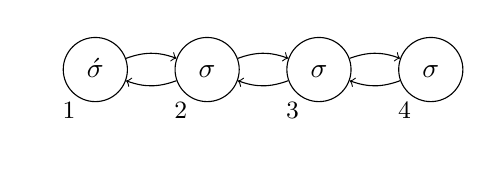
\begin{tikzpicture}[->, baseline=(m-1-1.base)]
    \matrix (m)
    [matrix of nodes, column sep=.75em, %row sep = -.3em,
     nodes={circle,text height=.75em, text depth = 2pt, text width = 1em, draw, align=center}]
    {
      \node(m-1-1)[label={[label distance=-.5em]260:{\small $1$}}]{$\ass$}; &
      \node(m-1-2)[label={[label distance=-.5em]260:{\small $2$}}]{$\sig$}; &
      \node(m-1-3)[label={[label distance=-.5em]260:{\small $3$}}]{$\sig$}; &
      \node(m-1-4)[label={[label distance=-.5em]260:{\small $4$}}]{$\sig$}; \\
    };
    \path(m-1-1) edge[bend left=20] (m-1-2);
    % \draw(m-1-1) to [bend left=45] (m-1-3);
    % \draw(m-1-1) to [bend left=45] (m-1-4);
    \path(m-1-2) edge[bend left=20]  (m-1-3);
    % \draw(m-1-2) to [bend right=45] (m-1-4);
    \path(m-1-3) edge[bend left=20]  (m-1-4);
    \path(m-1-4) edge[bend left=20]  (m-1-3);
    \path(m-1-3) edge[bend left=20]  (m-1-2);
    \path(m-1-2) edge[bend left=20]  (m-1-1);
  \end{tikzpicture}
 \label{exmodeloutput}
\end{exe}

\noindent
Notably, the transduction in (\ref{exampleoutput}) describes an initial stress input-output mapping not just for the strings in (\ref{exmodel}) and (\ref{exmodeloutput}), but for \textit{any} input string of syllables. 

The function just described is \textit{quantifier-free} (QF). Without invoking logical quantifiers $\exists$ or $\forall$, there is no way to reference positions that are an unbounded distance away from another position. For phonology, this is appropriate in many cases -- \citet{chandlee14} shows that a range of ``basic'' phonological processes are QF-definable. 

But not all phonological processes are local in this sense -- including stress assignment. In languages where stress iterates throughout a word, placement of stress cannot be defined by making local reference to a position in the input. Instead, I adopt a \textit{least-fixed point} logic \citep[LFP]{libkin04} that is modified to be QF. LFP logic defines transductions that recursively apply to their own output until convergence -- when a further application of the function would not result in changes. While full LFP logic is more powerful than first-order logic, the restriction to QFLFP transductions only limits the power by preserving a well-defined notion of locality in the definitions. An additional restriction is that, within a single defintion, an LFP may reference the predecessor function \textit{or} the successor function -- but not both. This restriction, while stipulative, is principled -- allowing the use of both in the same definition extends the power of the logic beyond the sequential class, which is unnecessary for most phonological processes \citep{chandlee14,chandJardSeq}.% and allows for definition of pathological mappings in, for example, tone \citep{kojAMP}.


\subsection{The sequential class and phonology}
 
QFLFP transductions are able to describe a great majority of phonological processes because they describe the \textit{sequential} class of functions \citep{chandJardSeq}. The sequential class of functions \citep{mohiri97} is relevant to phonology. It is properly \textit{sub-regular}, the regular class being a proposed boundary for phonology in general \citep{johnson72,kaplankay,heinz15}. It is an important division in the space of possible functions that includes many phonological patterns and excludes many non-phonological ones \citep{heinzlai13,chandlee14,jardine16}. The hope, then, is that QFLFP descriptions of phonological patterns will provide a rigorous, well-defined characterization that any particular theory of linguistics can make use of. It is shown in the following section that all quantity insensitive and most quantity sensitive stress assignment is QFLFP describable and thus sequential.

There are, however, some phonological mappings that are not sequential. Stem-control harmony \citep{heinzlai13}, as well as unbounded tonal plateauing, harmony in Yaka, and Sanskrit $n$-retroflexion \citep{jardine16}, are all provably non-sequential. Given how heavy the scale is tilted in the direction of sequentiality in phonology, these patterns appear quite exceptional, and are worthy of attention. It will be shown below that \textit{default-to-same} quantity sensitive stress patterns are not sequential, and so warrant further investigation as well. 

In the next section, I take up an analysis of different stress patterns, using QFLFP transductions between an input and output signature to define a stress assignment function.

\section{Analysis: Quantity Insensitive Stress}

In Quantity Insensitive (QI) stress languages, stress is placed in a predictable location given a word of any length, regardless of any properties the syllables in the word may have. I show that a wide range of QI patterns are describable with QFLFP transductions from an input signature to an output signature. For QI languages, the input signature is $S = \lbrace P_\sig, \; s, \; p \rbrace $ and the output signature is $S' = \lbrace P'_\ass, \; P'_\sig, \; s', \; p' \rbrace$. The only difference is the addition of unary predicate $P'_\ass$, which labels an element as stressed.

\subsection{Non-iterative}

Non-iterative stress patterns, sometimes called ``single stress'' \citep{gordon2002}, place only one stress in a fixed location. There are five attested patterns of this type -- initial (Nenets \citep{decsy66}); peninitial (Lakota \citep{boas41}); antepenultimate (Macedonian \citep{horace52}); penultimate (Albanian \citep{hetzer78}); and final (Atayal \citep{egerod66}). 

As stress assignment in these languages is non-iterative, there is no need to appeal to LFP logic. Transductions for non-iterative languages are simply QF. Consider the definition in (\ref{exampleoutput}), for example, partially repeated here\footnote{As the order of elements is always preserved from the input the output, I will not repeat the definitions for successor and predecessor functions.}:

\begin{exe}
\item $\begin{array}{l}
   P'_\ass(x) \deq  p(x) \approx x  \\
   P'_\sig(x) \deq  \neg p(x) \approx x  
     
\end{array} $
\label{singledef}
\end{exe}

\noindent
These formulae define an ``initial stress'' function -- a transduction that places stress on the first element in a string. Notice it does so without quantifiers or any reference to an LFP operator -- it is QF. The example below shows what this looks like as a mapping from an input string to an output string.

\begin{exe}

\item 
$\begin{array}[t]{lll}
  	\sig\sig\sig\sig                 & \mapsto & \brass\sig\sig\sig                 \\

  	
 	\end{array}$
 	\label{singlestressmap}
\end{exe}	
 	
Evaluating each element in the string as $x$, $P'_\ass(x)$ is only true for one element -- the first. This is the case for a string of any length over the input signature, not only this four-syllable example. Conversely, $P'_\sig(x)$ is true for every non-first element in the string, regardless of the length of the string. In this way, the definition of the logical transduction in (\ref{singledef}) describes an initial stress function appropriate for describing any language that displays an initial stress pattern. 

While the explicit definition in (\ref{singledef}) is informative, it is also useful to create user-defined predicates that make other, more complex definitions easier to understand. Examples of some useful predicates are shown in (\ref{usepred1}):

\begin{exe}
\item $\begin{array}{l}
   first(x) \deq  p(x) \approx x  \\
   last(x) \deq s(x) \approx x \\
   only(x) \deq first(x) \land last(x)
\end{array} $
\label{usepred1}
\end{exe}

\noindent
It is important to remember what is ``under the hood'' of user-defined predicates, but they are great aids in understanding the more complicated transductions described in later sections of this paper.

Another non-iterative pattern is the penultimate pattern. Penultimate stress targets the second to last syllable in a word. A QF transduction describing this pattern is given in (\ref{penultdef}):

\begin{exe}
\item $\begin{array}{l}
   P'_\ass(x) \deq  (last(s(x)) \land \neg last(x)) \lor only(x)  \\
  % P'_\sig(x) \deq  \neg p(x) \approx x  
     
\end{array} $
\label{penultdef}
\end{exe}
 	
\noindent 
The first disjunct refers to exactly the penultimate position in a string. Since the successor function is a total function i.e. the last element is also its own successor, the definition must also include a $\neg last(x)$ so that stress is not applied to the final syllable as well. The $only(x)$ disjunct ensures that a monosyllable is stressed as well -- the first disjunct alone would prevent this.

Again, this definition can be distilled into a useful predicate $penult(x)$, resulting in the following full definition of penultimate stress:

\begin{exe}
\item $\begin{array}{l}
   penult(x) \deq  (last(s(x)) \land \neg last(x)) \lor only(x)  \\
   P'_\ass(x) \deq penult(x)\\
   P'_\sig(x) \deq  \neg penult(x)  
     
\end{array} $
\label{penultpred}
\end{exe}

\noindent
Just as above in (\ref{singlestressmap}) for initial stress, this transduction maps any input string of syllables defined with our input signature to a string of syllables in the output where the penultimate syllable is stressed (ignoring the monosyllable). $P'_\ass(x) \deq penultimate(x)$ is true only of the penultimate syllable, and $P'_\sig(x) \deq \neg penultimate(x)$ is true of any non-penultimate syllable. 

\begin{exe}

\item 
$\begin{array}[t]{lll}
  	\sig\sig\sig\sig                 & \mapsto & \sig\sig\brass\sig                 \\
 	\end{array}$
 	\label{penultstressmap}
\end{exe}

For any of the five attested non-iterative stress patterns, there is a QF transduction describing the application of stress to a string of syllables. Rather than explicitly describing the remaining three, I add them to the list of user-defined predicates in (\ref{usepred1}), updated in (\ref{usepred2}): 


\begin{exe}

\item $\begin{array}{rl}
   first(x) \deq &  p(x) \approx x  \\
   peninitial(x) \deq & (first(p(x)) \land \neg first(x)) \lor only(x) \\
   penult(x) \deq & (last(s(x)) \land \neg last(x)) \lor only(x) \\
   antepenult(x) \deq & (last(s(s(x))) \land \neg penult(x) \land \neg last(x))\lor \\
    &   (first(x) \land penult(x)) \lor only(x)\\
   last(x) \deq & s(x) \approx x \\
   only(x) \deq & first(x) \land last(x)
\end{array} $
\label{usepred2}
\end{exe}

\noindent
Each of the first five predicates listed describes a QF transduction corresponding to placement of stress in non-iterative QI stress languages. They will prove useful in defining iterative stress patterns, as the iteration in all cases originates from one of the five positions the predicates describe.

Showing that the stress assignment function for these types of languages is QF has important theoretical implications. Any linguistic theory of word stress in non-iterative QI languages need not posit an input-output function that exceeds the QF boundary. I now turn to iterative stress patterns. 

\subsection{Iterative}

In iterative stress languages, stress is applied throughout the word, often skipping over a syllable before continuing. Consider the stress pattern of Pintupi \citep{hansen69}:

	\begin{exe}
	\item
  	Pintupi:       
  	$\ass, \; \tr, \; \tr\sig, \; \tr\tr, \; \tr\tr\sig, \; \tr\tr\tr, \; \tr\tr\tr\sig, \; \tr\tr\tr\tr   $
  	\end{exe}

\noindent 	
Stress starts at the left edge, from where it spreads to every other syllable thereafter excluding the final syllable. This kind of stress assignment is unbounded in the sense that the number of stresses grows as the length of the word grows. As such, a QF transduction is not enough to describe iterative stress. QFLFP, however, captures these types of patterns with recursive output structure definitions in a way that is still local. The definitions refer to a point in the output that is stressed after one pass of the transduction (the first syllable in the Pintupi example). Further stresses then iterate from there to some other position (no farther than 3 positions is ever needed) -- a third stress can iterate from the second, a fourth from the third, and so on.

The first group of patterns to examine are the non-exhaustive patterns, so-called because parsing to feet is not exhaustive in these languages in theories that employ metrical feet. This allows for lapses in stress -- gaps of two syllables where no stress occurs. There are four possible footing patterns in this category, three of which are attested, shown here (L-R trochees: Pintupi \citep{hansen69}; L-R iambs: Araucanian \citep{echev&cont65}; R-L trochees: Warao \citep{osborn66}; R-L iambs: \textit{unattested}):

 \begin{exe}
 \item	$\begin{array}[t]{llll}
  	\tm{L-R troch}   & \tm{L-R iamb}   &   \tm{R-L troch}  & \tm{R-L iamb}       \\
  	\ass             & \ass            &   \ass            & \ass                \\
  	\tr              & \im             &   \tr             & \im                 \\
  	\tr\sig          & \im\sig         &   \sig\tr         & \sig\im             \\
  	\tr\tr           & \im\im          &   \tr\tr          & \im\im              \\
  	\tr\tr\sig       & \im\im\sig      &   \sig\tr\tr      & \sig\im\im          \\
  	\tr\tr\tr        & \im\im\im       &   \tr\tr\tr       & \im\im\im           \\
  	\tr\tr\tr\sig    & \im\im\im\sig   &   \sig\tr\tr\tr   & \sig\im\im\im       \\
  	\tr\tr\tr\tr     & \im\im\im\im    &   \tr\tr\tr\tr    & \im\im\im\im
  	
 	\end{array}$
 	\label{iterativenonex}
\end{exe}

\noindent
Consider the Pintupi example. A transduction describing a non-exhaustive left-to-right trochaic stress assignment function is as follows:

\begin{exe}
\item

 $\begin{array}[t]{rl} 
 P'_\ass(x) \deq & [{\tiny{\texttt{lfp}}} first(y) \lor A(p(p(y)) \land \neg peninitial(y))](x) \land \\
                              & \neg( last(x) \land \neg only(x)) \\
  P'_\sig(x) \deq & [{\tiny{\texttt{lfp}}} peninitial(y) \lor A(p(p(y)))](x) \land \\
  & (last(x) \land \neg only(x))
  \end{array}$ 
  \label{pintdef}
\end{exe}

\noindent
 The first disjunct inside of the LFP establishes the ``base case'' of stress -- the starting point from which stress iterates outward. In Pintupi, this is the first syllable. All QFLFP definitions establish a base case that is first added to the LFP set. The second disjunct introduces the special set predicate $A$. This is what allows for recursive, local definitions based on the output. If a certain element is being evaluated as $y$, it checks the element obtained by double application of the predecessor function -- the element two positions to its left. If that element is in the set produced by the LFP operator, then $y$ is added to the set as well. There is an additional condition that $y$ not be peninitial -- as the $p$ and $s$ functions are total functions, applying $p$ twice to the peninitial position would return the first position. But since the first syllable is always in the LFP set, the formula would hold true for the peninitial, and it would be stressed as well, even though this is not what is observed in the actual stress pattern. So this is ruled out via the $\neg peninitial(y)$ conjunct. The final conjunct prevents the final syllable from ever being stressed as long as it is not the only syllable (not wanting to prevent stress assignment in the monosyllabic form).
 
 The intuition is that anything that meets the conditions of the first formula will be stressed in the output. Some number of elements (syllables) is added to the LFP set via the base case or via the recursive set predicate, modulo restrictions either inside the LFP definition -- preventing them from being added to the set at all -- or outside, preventing them from entering the unary relation $P'_\ass(x)$ even if they are in the LFP.  The following shows how this occurs in six and seven syllable forms:
 
 \begin{exe} 
 \item
 $\begin{array}[t]{llll}
  	1. &\sig\sig\sig\sig\sig\sig & \mapsto & \brass\sig\sig\sig\sig\sig            \\
  	2. &\brass\sig\sig\sig\sig\sig & \mapsto & \brass\sig\brass\sig\sig\sig        \\
  	3. &\brass\sig\brass\sig\sig\sig & \mapsto & \brass\sig\brass\sig\brass\sig         \\
  	4. &\brass\sig\brass\sig\brass\sig\sig & \mapsto & \brass\sig\brass\sig\brass\sig   \\ 
  \end{array}
  \hspace{1em}
  \begin{array}[t]{llll}
  	1. &\sig\sig\sig\sig\sig\sig\sig & \mapsto & \brass\sig\sig\sig\sig\sig\sig     \\
  	2. &\brass\sig\sig\sig\sig\sig\sig & \mapsto & \brass\sig\brass\sig\sig\sig\sig                \\
  	3. &\brass\sig\brass\sig\sig\sig\sig & \mapsto & \brass\sig\brass\sig\brass\sig\sig         \\
  	4. &\brass\sig\brass\sig\brass\sig\sig & \mapsto & \brass\sig\brass\sig\brass\sig\sig   \\ 
  	 	\end{array}$
  	 	\label{pinttrans}
\end{exe}

\noindent
After the first pass of the transduction, the first syllable is labeled as stressed. It is the only element in the string that meets the conditions of the formula in (\ref{pintdef}). At the second pass, the third syllable satisfies the conditions of the $A(p(p(y)) \land \neg peninitial(y))$ disjunct. The syllable two positions to the left is in the set, and so the third syllable is added as well. It meets all conditions of the formula, and so is labeled as stressed. On the third pass, the same is true of the fifth syllable, so it is stressed too. On the fourth pass, no more elements are added to the LFP -- the function has converged on correct outputs for a six and seven syllable word in Pintupi. It is in this way, through local recursive output definitions, that QFLFP is able to capture iterative stress patterns. The transduction described in (\ref{pintdef}) will take a string over the input signature of any length and apply a Pintupi-like stress pattern. There is a QFLFP transduction describing all four of the non-exhaustive patterns in (\ref{iterativenonex}) (see Appendix). 

In the remainder of this section, I briefly show QFLFP transductions for two other categories of QI iterative stress patterns. The first is the exhaustive patterns, so called because they do not allow unparsed syllables in theories that use feet. This can result in a stress clash, where two stresses occur next to each other. Again assuming a foot-parsing method of categorization, there are four possible patterns, all attested (L-R trochees: Murinbata \citep{street81}; L-R iambs: Ojibwa \citep{kaye73}; R-L trochees: Biangai \citep{dubert73}; R-L iambs: Weri \citep{boxwell66}).

 \begin{exe}
 \item	$\begin{array}[t]{llll}
  	\tm{L-R troch}   & \tm{L-R iamb}   &   \tm{R-L troch}  & \tm{R-L iamb}       \\
  	\ass             & \ass            &   \ass            & \ass                \\
  	\tr              & \im             &   \tr             & \im                 \\
  	\tr\ass          & \im\ass         &   \ass\tr         & \ass\im             \\
  	\tr\tr           & \im\im          &   \tr\tr          & \im\im              \\
  	\tr\tr\ass       & \im\im\ass      &   \ass\tr\tr      & \ass\im\im          \\
  	\tr\tr\tr        & \im\im\im       &   \tr\tr\tr       & \im\im\im           \\
  	\tr\tr\tr\ass    & \im\im\im\ass   &   \ass\tr\tr\tr   & \ass\im\im\im       \\
  	\tr\tr\tr\tr     & \im\im\im\im    &   \tr\tr\tr\tr    & \im\im\im\im
  	
 	\end{array}$
 	\label{iterativeex}
\end{exe}

\noindent
It is apparent that these are minor variations on the non-exhaustive patterns. In fact, application of stress is less restrictive, and so the definitions of the transductions are simpler. Consider the case of Murinbata, the exhaustive reflex of Pintupi:

\begin{exe}

\item
  {\small{$ P'_\ass(x) \deq [{\tiny{\texttt{lfp}}} first(y) \lor A(p(p(y)) \land \neg peninitial(y))](x) $ 
   
   
   $ P'_\sig(x) \deq [{\tiny{\texttt{lfp}}} peninitial(y) \lor A(p(p(y)))](x) $ }}\\



$\begin{array}[t]{llll}
  	1. &\sig\sig\sig\sig\sig\sig & \mapsto & \brass\sig\sig\sig\sig\sig            \\
  	2. &\brass\sig\sig\sig\sig\sig & \mapsto & \brass\sig\brass\sig\sig\sig        \\
  	3. &\brass\sig\brass\sig\sig\sig & \mapsto & \brass\sig\brass\sig\brass\sig         \\
  	4. &\brass\sig\brass\sig\brass\sig\sig & \mapsto & \brass\sig\brass\sig\brass\sig   \\ 
  \end{array}
  \hspace{1em}
  \begin{array}[t]{llll}
  	1. &\sig\sig\sig\sig\sig\sig\sig & \mapsto & \brass\sig\sig\sig\sig\sig\sig                 \\
  	2. &\brass\sig\sig\sig\sig\sig\sig & \mapsto & \brass\sig\brass\sig\sig\sig\sig                \\
  	3. &\brass\sig\brass\sig\sig\sig\sig & \mapsto & \brass\sig\brass\sig\brass\sig\sig         \\
  	4. &\brass\sig\brass\sig\brass\sig\sig & \mapsto & \brass\sig\brass\sig\brass\sig\brass   \\ 
  	5. &\brass\sig\brass\sig\brass\sig\brass & \mapsto & \brass\sig\brass\sig\brass\sig\brass \\
  	 	\end{array}$
 \label{murindeftrans} 	 	
 \end{exe}

\noindent
The definition of the stress assignment function for Murinbata is only the LFP portion of the definition for Pintupi (\ref{pintdef}), minus the conjunct banning final stress. As shown in the diagram of the transduction, stress iterates onto a syllable two positions away on each pass until convergence on the correct output forms for the language. See the Appendix for QFLFP definitions of the remaining three exhaustive patterns.

A final group of iterative QI patterns to be examined are the ``internal lapse'' or ``bidirectional'' patterns. These feature a stress fixed at one edge, with other stresses iterating from the opposite edge. When this iteration would place a stress next to the opposite edge fixed stress, this is avoided instead, creating an internal lapse. Two examples are shown here, with foot structure shown to give a better sense of the pattern (Garawa \citep{furby74}; Piro \citep{matteson65}):

 \begin{exe}
 \item	$\begin{array}[t]{llll}
  	\tm{Garawa, footed}   & \tm{Garawa, unfooted}   &   \tm{Piro, footed}     & \tm{Piro, unfooted}       \\
  	(\ass)                & \ass                    &   (\ass)                & \ass                \\
  	(\tr)                 & \tr                     &   (\tr)                 & \tr                 \\
  	(\tr)\sig             & \tr\sig                 &   \sig(\tr)             & \sig\tr             \\
  	(\tr)(\tr)            & \tr\tr                  &   (\tr)(\tr)            & \tr\tr              \\
  	(\tr)\sig(\tr)        & \tr\sig\tr              &   (\tr)\sig(\tr)        & \tr\sig\tr          \\
  	(\tr)(\tr)(\tr)       & \tr\tr\tr               &   (\tr)(\tr)(\tr)       & \tr\tr\tr           \\
  	(\tr)\sig(\tr)(\tr)   & \tr\sig\tr\tr           &   (\tr)(\tr)\sig(\tr)   & \tr\tr\sig\tr       \\
    (\tr)(\tr)(\tr)(\tr)  & \tr\tr\tr\tr            &   (\tr)(\tr)(\tr)(\tr)  & \tr\tr\tr\tr
  	
 	\end{array}$
 	\label{bidirect}
\end{exe}

\noindent
Though on the surface these may appear more complex than the other iterative patterns seen thus far, they are equally amenable to a QFLFP defintion. Take Garawa, for example. The definition of the stress assignment function and an example transduction are as follows:

\begin{exe}
 \item
 {\small{$ P'_\ass(x) \deq first(x) \land ([{\tiny{\texttt{lfp}}} penult(y) \lor A(s(s(y)))](x) \land \neg peninitial(x)) $ 
   
   
   $ P'_\sig(x) \deq peninitial(x) \land ([{\tiny{\texttt{lfp}}}last(y) \lor A(s(s(y)))](x) \land \neg first(x))$ }}\\



$\begin{array}[t]{llll}
  	1. &\sig\sig\sig\sig\sig\sig & \mapsto & \brass\sig\sig\sig\brass\sig                 \\
  	2. &\sig\sig\sig\sig\sig\sig & \mapsto & \brass\sig\brass\sig\brass\sig         \\
  	3. &\sig\sig\sig\sig\sig\sig & \mapsto & \brass\sig\brass\sig\brass\sig   \\ 
  \end{array}
  \hspace{1em}
  \begin{array}[t]{llll}
  	1. &\sig\sig\sig\sig\sig\sig\sig & \mapsto & \brass\sig\sig\sig\sig\brass\sig                 \\
  	2. &\sig\sig\sig\sig\sig\sig\sig & \mapsto & \brass\sig\sig\brass\sig\brass\sig                \\
  	3. &\sig\sig\sig\sig\sig\sig\sig & \mapsto & \brass\sig\sig\brass\sig\brass\sig        \\
  	 	\end{array}$ 
\label{gardeftrans} 
\end{exe}


\section{Analysis: Quantity Sensitive stress}

\section{Discussion}

\section{Conclusion}






\bibliography{refs}
\bibliographystyle{apalike} 

\end{document}
